\chapter{Manual de usuario de la aplicación móvil}
\label{chap:application}

\section{Acceso a la aplicación}

Al iniciar la aplicación se muestra la ventana principal [Figura~\ref{fig:main_page}] la cual contiene una breve descripción sobre su uso y configuración. Desde esta ventana se pueden realizar dos acciones:
\begin{itemize}
    \item Acceder a la ventana de configuración
    \item Iniciar la prueba
\end{itemize}

\begin{figure}[!h]
    \centering
    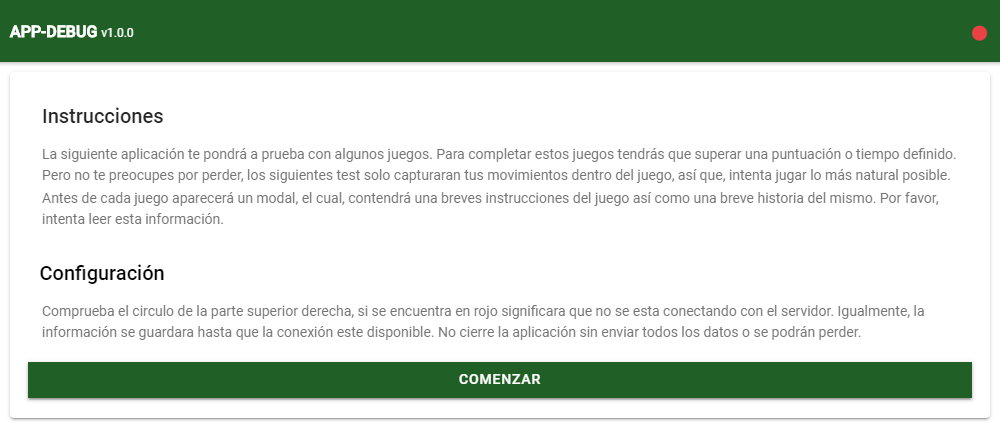
\includegraphics[width=0.8\textwidth, keepaspectratio]{imaxes/application/main_page.png}
    \caption{Ventana principal}
    \label{fig:main_page}
\end{figure}

\section{Configuración de la aplicación}

Para acceder a la pantalla de configuración es necesario realizar un patrón, que consiste en tocar las cuatro esquinas de la pantalla. Al realizar el patrón se mostrará la configuración de la aplicación [Figura~\ref{fig:config_page}]. En esta ventana se puede configurar algunos de los aspectos de la aplicación como tiempo de la aplicación y la dirección del servidor. Además de la configuración también se muestran los datos actuales de la aplicación y un registro de eventos.

\begin{figure}[!h]
    \centering
    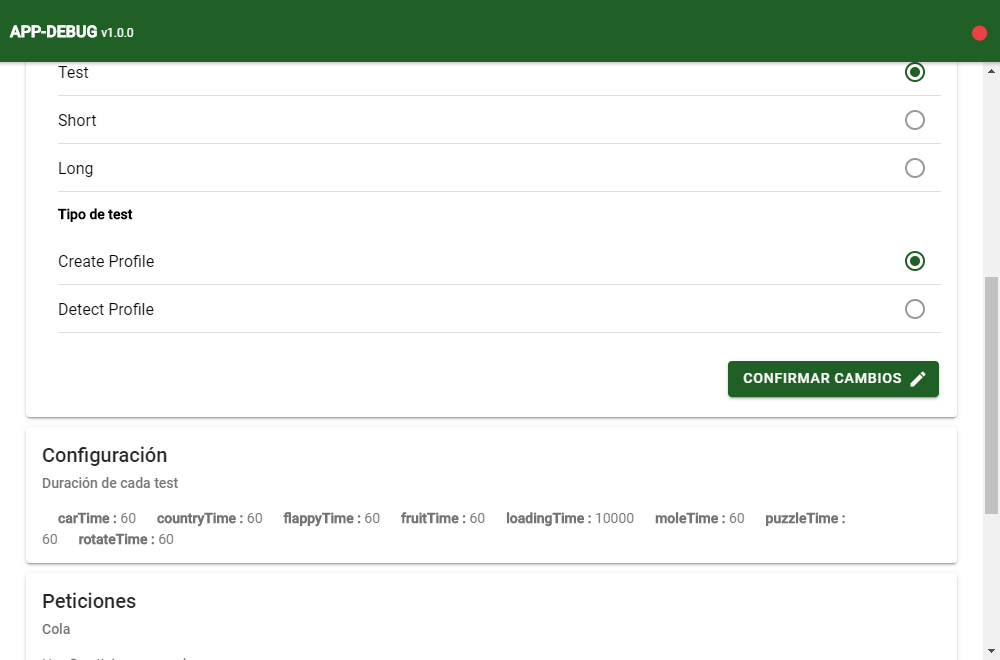
\includegraphics[width=0.8\textwidth, keepaspectratio]{imaxes/application/config_page.png}
    \caption{Menú de configuración}
    \label{fig:config_page}
\end{figure}

\newpage
\section{Inicio de la prueba}

Para iniciar la prueba solo es necesario presionar el botón \textbf{COMENZAR} y a continuación se abrirá un dialogo donde tendremos que introducir el nombre de usuario. [Figura~\ref{fig:login_page}]. 

\begin{figure}[!h]
    \centering
    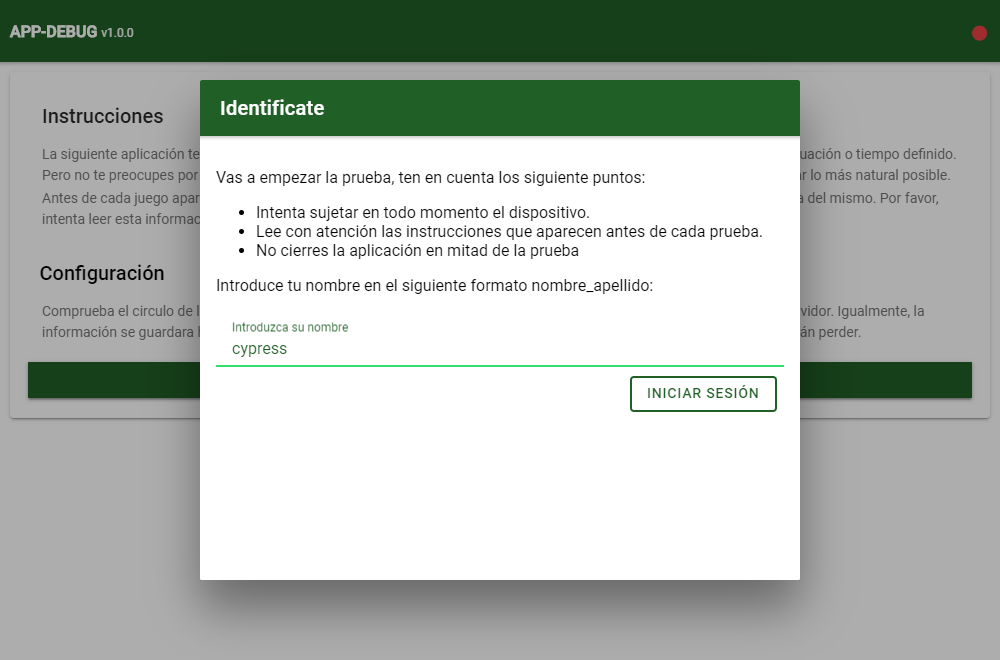
\includegraphics[width=0.6\textwidth, keepaspectratio]{imaxes/application/login_page.png}
    \caption{Ventana de login}
    \label{fig:login_page}
\end{figure}

\subsection{Desafíos}

\subsubsection{Puzzle Sliding}

Esta primera prueba [Figura~\ref{fig:puzzle_page}] consiste en resolver el puzzle que se muestra en pantalla, realizando movimientos de deslizamiento, en un tiempo límite establecido.

\begin{figure}[!h]
    \centering
    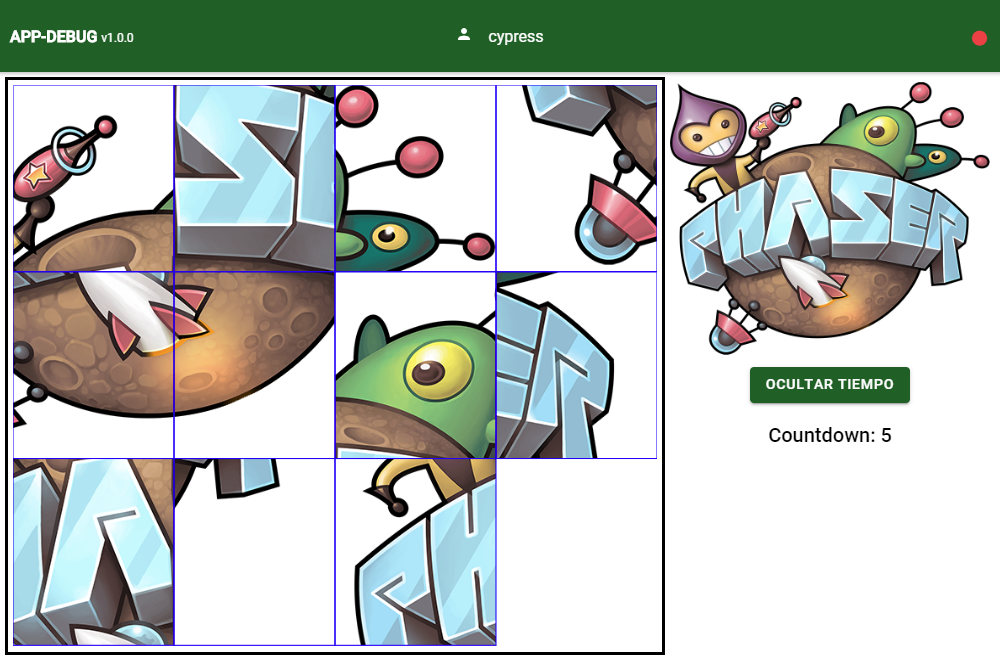
\includegraphics[width=0.6\textwidth, keepaspectratio]{imaxes/application/puzle-sliding-page.png}
    \caption{Ventana del juego de \textit{Puzzle Sliding}}
    \label{fig:puzzle_page}
\end{figure}

\subsubsection{Whack a mole}
En esta prueba [Figura~\ref{fig:mole_page}] tendremos que tocar la pantalla sobre los animales, los cuales aparecerán cada cierto tiempo.

\begin{figure}[H]
    \centering
    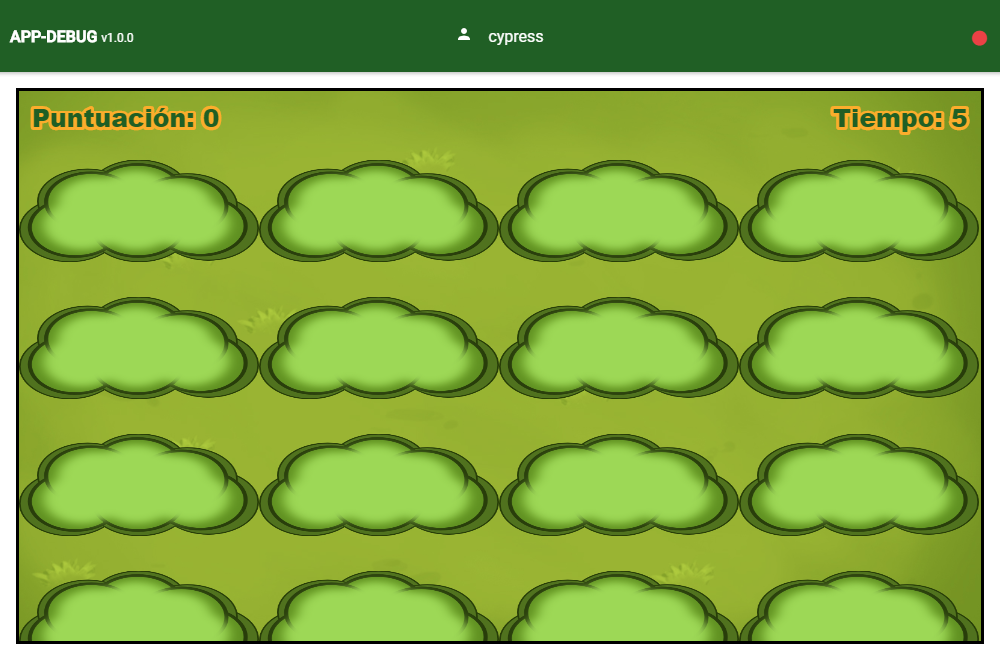
\includegraphics[width=0.7\textwidth, keepaspectratio]{imaxes/application/whack-mole-page.png}
    \caption{Ventana del juego de \textit{Whack a Mole}}
    \label{fig:mole_page}
\end{figure}

\subsubsection{Flappy Bird}
En esta prueba [Figura~\ref{fig:bird_page}] tendremos tocar la pantalla repetidamente, para intentar que el pájaro no choque contra las tuberías que irán apareciendo.

\begin{figure}[!h]
    \centering
    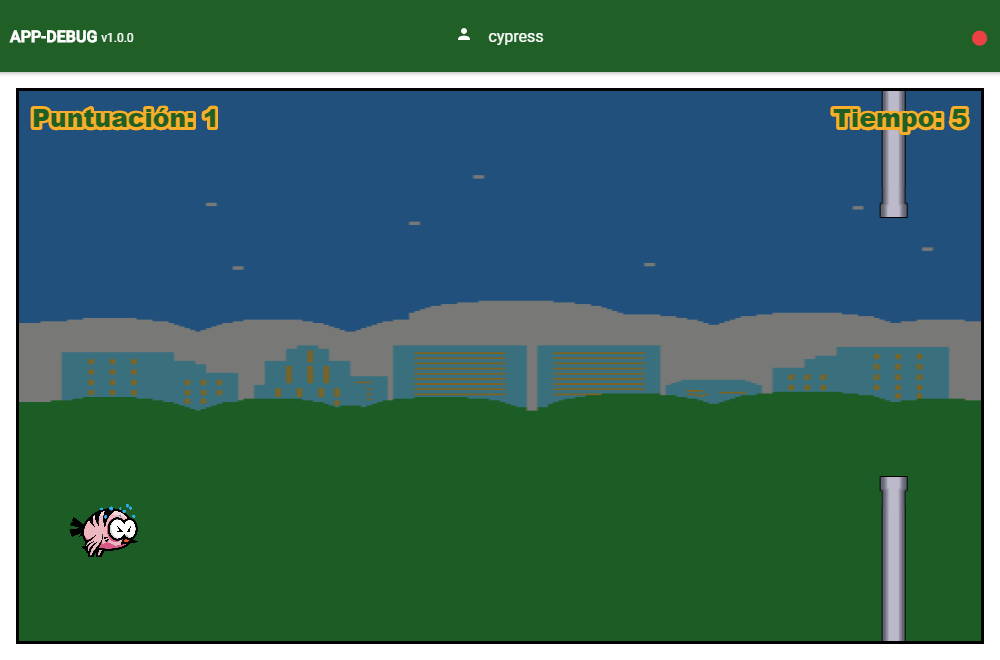
\includegraphics[width=0.7\textwidth, keepaspectratio]{imaxes/application/flappy-bird-page.png}
    \caption{Ventana del juego de \textit{Flappy Bird}}
    \label{fig:bird_page}
\end{figure}

\subsubsection{Fruit Ninja}
En esta prueba [Figura~\ref{fig:bird_page}] tendremos que delizar el dedo sobre la pantalla para cortar la fruta que vaya apareciendo.

\begin{figure}[!h]
    \centering
    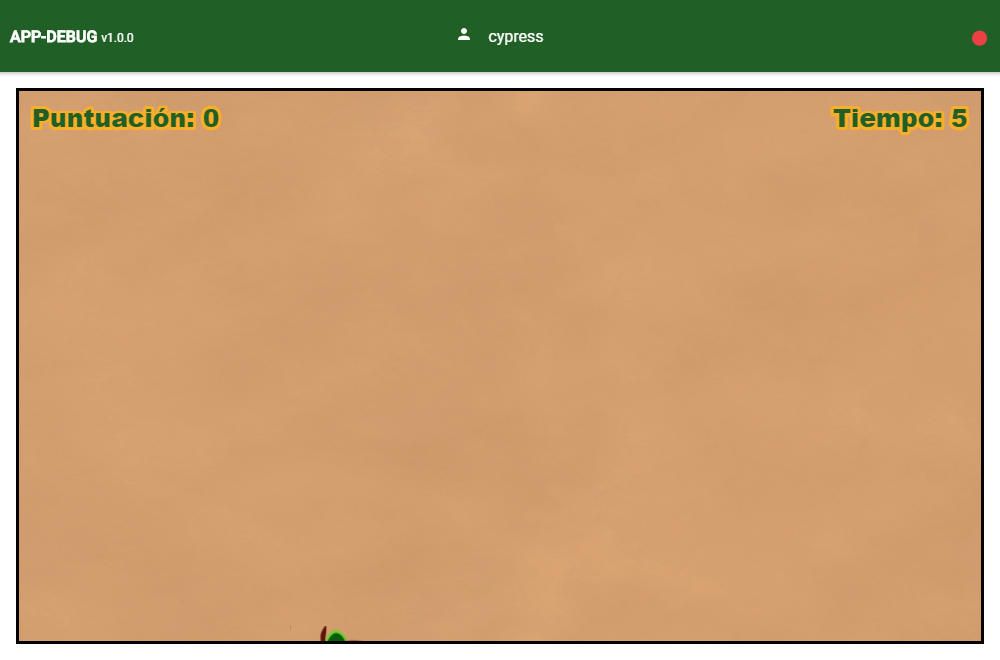
\includegraphics[width=0.7\textwidth, keepaspectratio]{imaxes/application/fruit-ninja-page.png}
    \caption{Ventana del juego de \textit{Fruit Ninja}}
    \label{fig:fruit_page}
\end{figure}

\subsubsection{Outrun}
En esta prueba [Figura~\ref{fig:bird_page}] tendremos que coger el dispositivo como si fuera el volante e intentar esquivar los obstaculos que irán apareciendo.

\begin{figure}[!h]
    \centering
    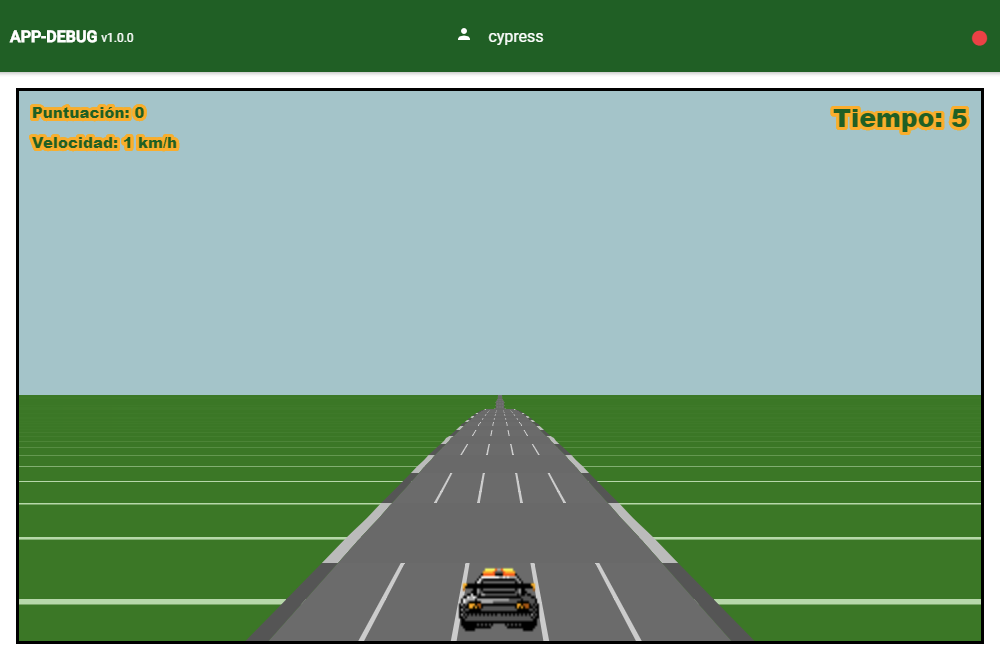
\includegraphics[width=0.7\textwidth, keepaspectratio]{imaxes/application/outrun-page.png}
    \caption{Ventana del juego de \textit{Outrun}}
    \label{fig:outrun_page}
\end{figure}

\subsubsection{Buscar Países}
En esta prueba [Figura~\ref{fig:search_page}] se nos muestra una lista de países ordenados alfabéticamente. El objetivo es buscar los países que se muestran en la parte superior izquierda.

\begin{figure}[!h]
    \centering
    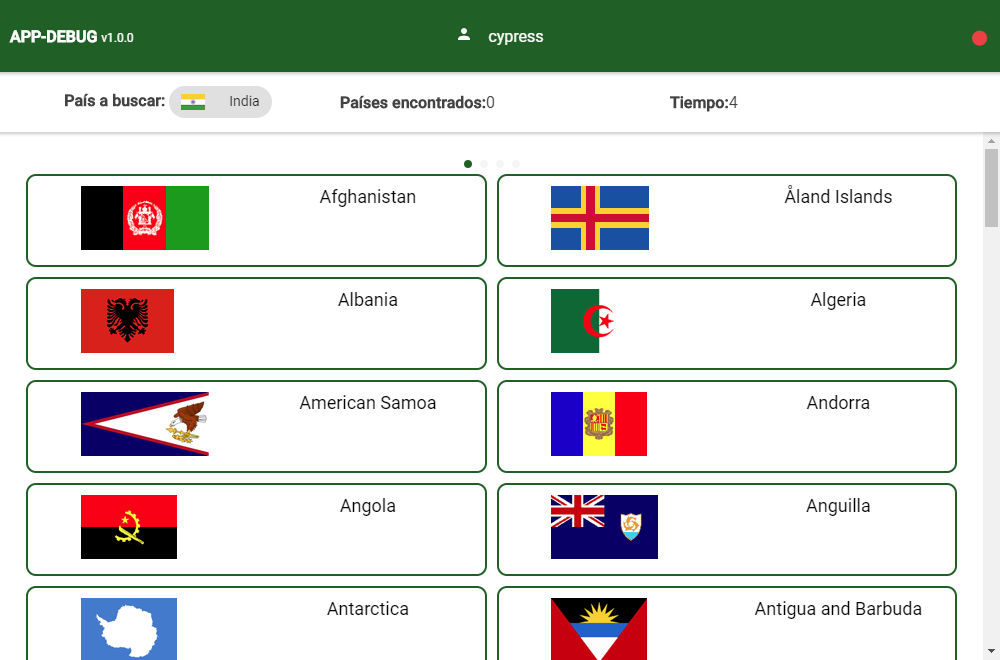
\includegraphics[width=0.7\textwidth, keepaspectratio]{imaxes/application/search-page.png}
    \caption{Ventana del juego de \textit{Buscar Países}}
    \label{fig:search_page}
\end{figure}

\subsubsection{Rotación}
En esta prueba [Figura~\ref{fig:rotate_page}] tendremos que hacer encajar las piezas y para ello tendremos que mover, rotar y escalar la pieza negra.

\begin{figure}[!h]
    \centering
    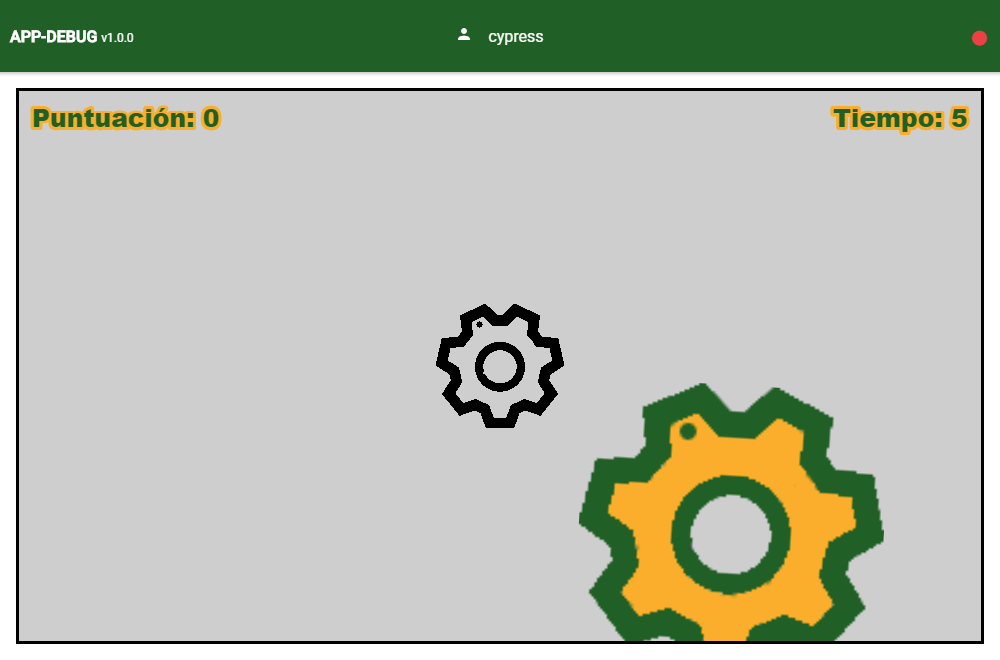
\includegraphics[width=0.7\textwidth, keepaspectratio]{imaxes/application/rotate-page.png}
    \caption{Ventana del juego de \textit{Rotación}}
    \label{fig:rotate_page}
\end{figure}


\subsection{Fin de la prueba}
Una vez finalizadas todas la pruebas la aplicación nos mostrara una tabla de puntuaciones [Figura~\ref{fig:score_page}] de todos los desafíos hechos. En esta ventana podremos volver al inicio pulsando el botón \textit{IR A INICIO}.

\begin{figure}[!h]
    \centering
    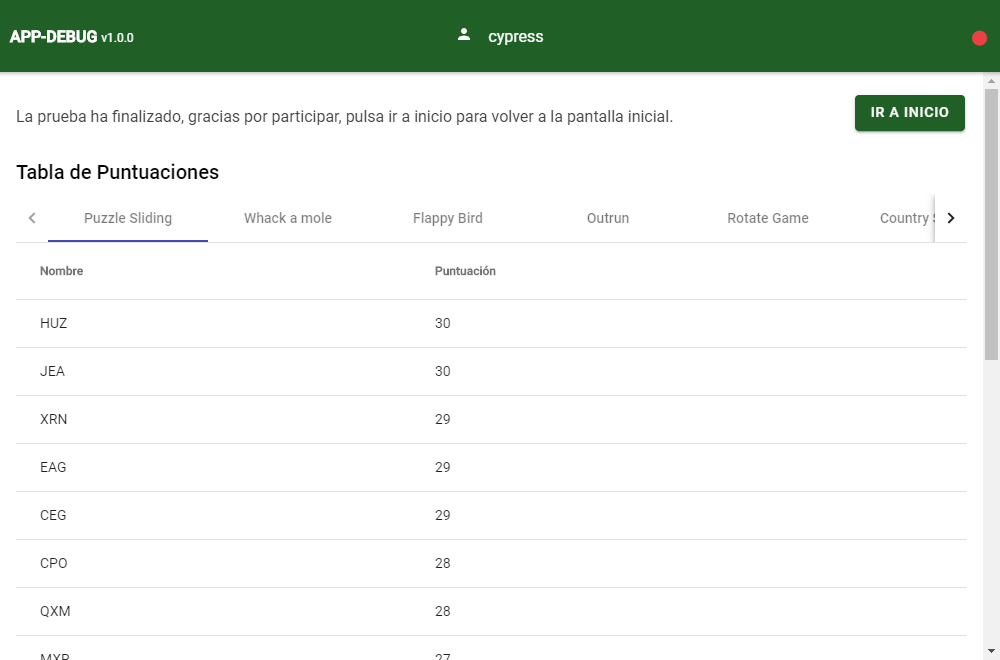
\includegraphics[width=0.7\textwidth, keepaspectratio]{imaxes/application/score-page.png}
    \caption{Ventana de puntuaciones}
    \label{fig:score_page}
\end{figure}